\documentclass{article}

\usepackage{geometry}
\usepackage{longtable}
\usepackage[dvipsnames,table]{xcolor}
\usepackage{fancyhdr}
\usepackage{xcolor}
\usepackage{graphicx}
\usepackage{hyperref}
\usepackage{float}
\usepackage{listings}
\usepackage{amssymb}
\usepackage{amsmath}
\usepackage{enumitem}
\usepackage{parskip}
\usepackage{booktabs}

% Choose paper size
\geometry{letterpaper, top=25.4mm, bottom=25.4mm, left=25.4mm, right=25.4mm}
%\geometry{a4paper, top=25.4mm, bottom=25.4mm, left=25.4mm, right=25.4mm}

\color{black}
\fancyhf{}
\renewcommand{\headrulewidth}{1pt}
\renewcommand{\footrulewidth}{1pt}

% Define standard IPF color palette
\definecolor{soft-sky-blue}{HTML}{B7DAEB}
\definecolor{orange}{HTML}{FF6633}
\definecolor{cool-grey}{HTML}{91A1B0}
\definecolor{black}{HTML}{000000}
\definecolor{space-blue}{HTML}{003366}
\definecolor{pigeon-blue}{HTML}{5F8396}
\definecolor{sage-green}{HTML}{95A077}
\definecolor{fire-yellow}{HTML}{F9A651}
\definecolor{apple-red}{HTML}{CC4200}
\definecolor{crockadile-green}{HTML}{718944}
\definecolor{slate-grey}{HTML}{607587}
\definecolor{fog-grey}{HTML}{E5E6E9}

% Define certification colors
\definecolor{cert-level-0}{HTML}{CC4200} % apple-red
\definecolor{cert-level-1}{HTML}{FF6633} % orange
\definecolor{cert-level-2}{HTML}{F9A651} % fire-yellow
\definecolor{cert-level-3}{HTML}{B7DAEB} % soft-sky-blue
\definecolor{cert-level-4}{HTML}{5F8396} % pigeon-blue
\definecolor{cert-level-5}{HTML}{718944} % sage-green

\hypersetup{hidelinks}
\pagestyle{fancy}
\pagenumbering{arabic}

\title{

\includegraphics[width=8cm] {images/Rocksavage_Tech_RGB_300.png}\vspace{50pt}
\vspace{10pt} \\
\textbf{Gpio \\
  Product User Guide} \\
{\small{\textcolor{slate-grey}{rocksavagetech.chiselWare.Gpio}}} \\
\vspace{20pt} IPF certified to level:
\textbf{\textcolor{cert-level-0}{0} }of 5 \\
\vspace{5pt}

\includegraphics[width=4cm] {images/uncertified.png}
}

\author{Abdelrahman Abbas, Ahmed Elmenshawi, Nick Allison, Jimmy Bright}

\fancyhead[L]{Gpio Users Guide}
\fancyhead[R]{\leftmark}
\fancyfoot[C]{Rocksavage Technology, Inc.~\copyright~2023}
\fancyfoot[R]{Page \thepage}

\begin{document}

\maketitle
\newpage
\tableofcontents 
\newpage


\section{Features}
The SPI (Serial Peripheral Interface) core is equipped with a variety of features that make it a versatile and efficient choice for synchronous serial communication in embedded systems. Below is a detailed list of its key features:

\begin{itemize}
    \item \textbf{Full Duplex, Three-Wire Synchronous Data Transfer:} Enables simultaneous transmission and reception of data, enhancing communication efficiency.
    \item \textbf{Master or Slave Operation:} The SPI core can function as either a master, initiating and controlling communication, or as a slave, responding to the master's commands.
    \item \textbf{LSb First or MSb First Data Transfer:} Flexibly configures the data transmission order based on the system requirements, supporting both Least Significant Bit (LSb) first and Most Significant Bit (MSb) first formats.
    \item \textbf{Programmable Bit Rates:} Allows customization of the SPI clock speed to match the performance needs of different peripherals and system constraints.
    \item \textbf{End of Transmission Interrupt Flag:} Notifies the system when a data transmission cycle is complete, facilitating efficient interrupt-driven communication.
    \item \textbf{Write Collision Protection:} Prevents data corruption by detecting and handling scenarios where multiple write attempts occur simultaneously.
    \item \textbf{Wake-up from Idle Mode:} Supports low-power operations by enabling the SPI core to wake up from idle states upon specific events or triggers.
    \item \textbf{Double-Speed Master SPI Mode:} Increases data throughput by doubling the SPI clock rate in master mode, enhancing overall system performance.
\end{itemize}

\section{Overview}
The Serial Peripheral Interface (SPI) core is a robust and high-speed synchronous communication protocol widely used in embedded systems. It facilitates reliable data exchange between a central controller (master) and various peripheral devices (slaves) such as sensors, memory modules, and other microcontrollers. The SPI core's flexibility in operating modes and data transfer configurations makes it suitable for a broad range of applications, from simple data logging to complex sensor networks.

Key aspects of the SPI core include:
\begin{itemize}
    \item \textbf{High-Speed Data Transfer:} SPI supports fast data rates, making it ideal for applications requiring rapid data exchange.
    \item \textbf{Full-Duplex Communication:} Allows simultaneous sending and receiving of data, optimizing communication efficiency.
    \item \textbf{Simple Hardware Interface:} Utilizes minimal wiring (typically three or four lines), reducing hardware complexity and saving valuable board space.
    \item \textbf{Scalability:} Can connect multiple slave devices to a single master, enabling scalable system designs.
\end{itemize}

\subsection{Use Cases}
The SPI core is employed in various scenarios, including:
\begin{itemize}
    \item \textbf{Interfacing with Sensors:} Communicates with high-precision sensors in automotive, industrial, and consumer electronics.
    \item \textbf{Memory Devices:} Interfaces with flash memory, EEPROMs, and other storage modules for data retention.
    \item \textbf{Display Modules:} Drives LCD, OLED, and other display technologies requiring efficient data streaming.
    \item \textbf{Communication Modules:} Connects with wireless modules like Bluetooth and Wi-Fi for data transmission.
\end{itemize}

% Block Diagram
\begin{figure}[H]
    \centering
    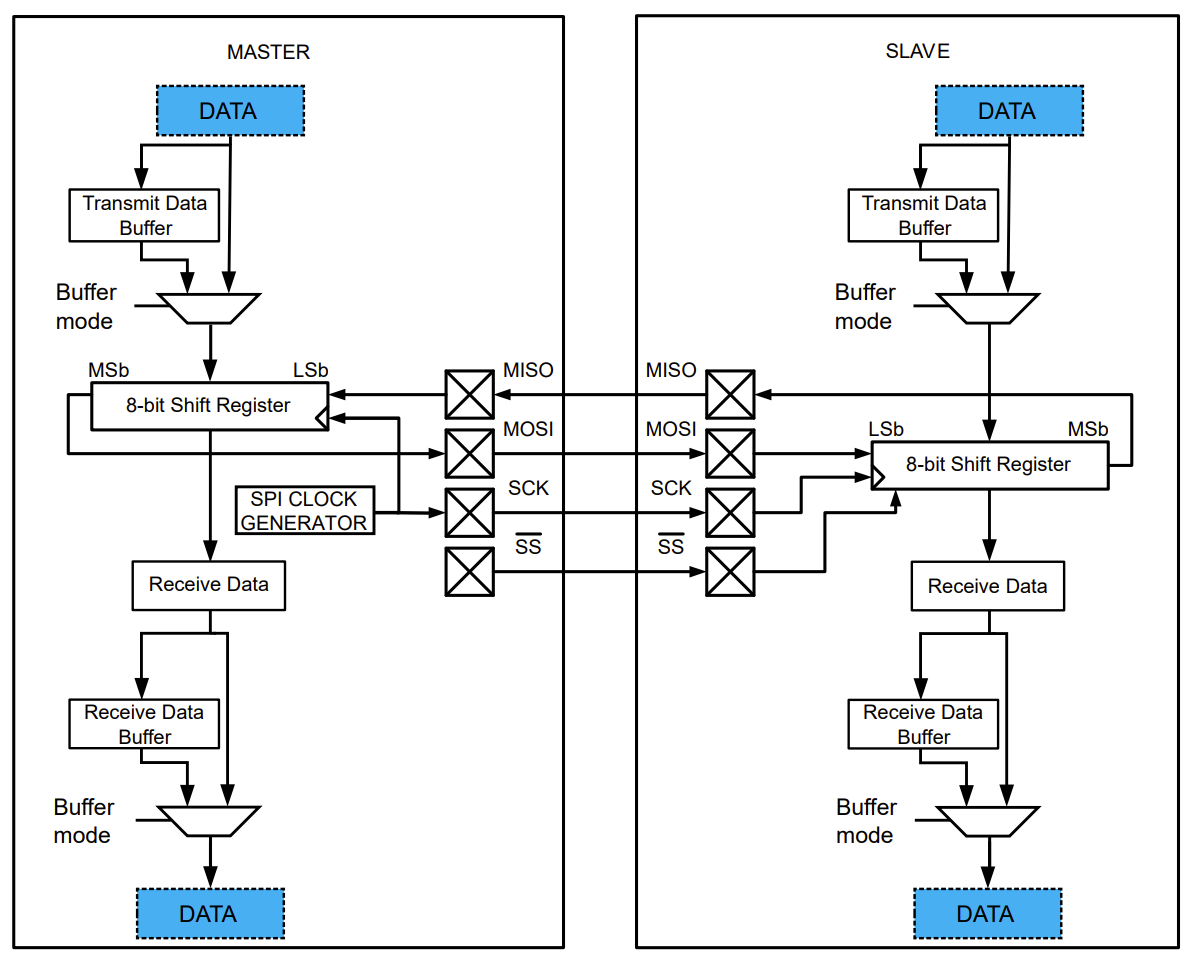
\includegraphics[width=0.8\textwidth]{images/spi_block_diagram.png}
    \caption{SPI Core Block Diagram}
    \label{fig:spi_block_diagram}
\end{figure}

\section{Functional Description}
The SPI core operates by shifting data in and out through an 8-bit shift register, enabling both transmission and reception of data bytes. Its functional versatility is achieved through configurable modes that determine its role as a master or slave, the data order, and the clock settings.

\subsection{Operation Modes}
\subsubsection{Master Mode}
In master mode, the SPI core takes charge of the communication process. It generates the serial clock signal (SCK) and manages the Slave Select (SS) lines to initiate and terminate communication with slave devices. The master controls the timing and synchronization of data transfers, ensuring orderly and efficient communication.

\subsubsection{Slave Mode}
Conversely, in slave mode, the SPI core responds to the master's commands. It does not generate the clock signal but instead listens for the SCK and SS signals from the master. Upon selection (when SS is active), the slave prepares to receive or transmit data as dictated by the master's operations.

\subsection{Data Transmission and Reception}
Data transmission in SPI is accomplished through simultaneous shifting of data out (MOSI) and shifting of data in (MISO). The shift registers ensure that each byte of data is accurately transferred between the master and slave devices.

\subsection{Clock Management}
The SPI core's clock management is pivotal for synchronization. In master mode, the core controls the SCK frequency and phase, ensuring that both master and slave devices operate in lockstep. The ability to double the clock speed in master mode further enhances data throughput when needed.

% Signal Diagram
% \begin{figure}[H]
%     \centering
%     \includegraphics[width=0.8\textwidth]{images/spi_signal_diagram.png}
%     \caption{SPI Signal Connections}
%     \label{fig:spi_signal_diagram}
% \end{figure}

\subsection{Signal Descriptions}
Effective communication in SPI hinges on the proper management of its signal lines. The SPI core utilizes four primary signals, each serving a distinct purpose in data exchange.

\begin{table}[H]
    \centering
    \caption{SPI Signal Descriptions}
    \begin{tabular}{@{}ccc@{}}
        \toprule
        \textbf{Signal} & \textbf{Master Mode} & \textbf{Slave Mode} \\ \midrule
        MOSI & Output & Input \\
        MISO & Input & Output \\
        SCK  & Output & Input \\
        SS   & Output & Input \\ \bottomrule
    \end{tabular}
    \label{tab:spi_signals}
\end{table}

\begin{itemize}
    \item \textbf{MOSI (Master Out Slave In):} Carries data from the master to the slave device. In master mode, this line is configured as an output, while in slave mode, it serves as an input.
    \item \textbf{MISO (Master In Slave Out):} Carries data from the slave to the master device. Conversely, this line is an input in master mode and an output in slave mode.
    \item \textbf{SCK (Serial Clock):} Generated by the master to synchronize data transmission. The clock signal dictates the timing of data bits being sent and received.
    \item \textbf{SS (Slave Select):} An active-low signal used by the master to select a specific slave device for communication. When SS is low, the corresponding slave device becomes active and engages in data exchange.
\end{itemize}

\section{Initialization}
Proper initialization of the SPI core is crucial to ensure reliable and efficient communication. The initialization process involves configuring the SPI core's operating parameters and enabling its functionality.

\subsection{Initialization Steps}
To initialize the SPI core for basic operation, follow these comprehensive steps:

\begin{enumerate}
    \item \textbf{Configure the SS Pin Direction:}
    \begin{itemize}
        \item Set the direction of the Slave Select (SS) pin as an output in the I/O port if operating in master mode.
        \item If in slave mode, configure the SS pin as an input to allow the master to select the slave device.
    \end{itemize}
    
    \item \textbf{Select Operation Mode:}
    \begin{itemize}
        \item Access the Control Register A (\texttt{CTRLA}).
        \item Set the \texttt{MASTER} bit to \texttt{1} for master mode or \texttt{0} for slave mode.
    \end{itemize}
    
    \item \textbf{Configure Clock Rate (Master Mode Only):}
    \begin{itemize}
        \item In master mode, set the \texttt{PRESC} bits to determine the SPI clock prescaler.
        \item Optionally, set the \texttt{CLK2X} bit to \texttt{1} to double the SPI clock rate after prescaling.
    \end{itemize}
    
    \item \textbf{Set Data Order:}
    \begin{itemize}
        \item Access the \texttt{DORD} bit in \texttt{CTRLA}.
        \item Set \texttt{DORD} to \texttt{0} for MSB first or \texttt{1} for LSb first data transmission.
    \end{itemize}
    
    \item \textbf{Enable Buffer Mode (Optional):}
    \begin{itemize}
        \item Access Control Register B (\texttt{CTRLB}).
        \item Set the \texttt{BUFEN} bit to \texttt{1} to enable buffer mode, allowing for enhanced data handling and buffering.
    \end{itemize}
    
    \item \textbf{Enable the SPI Core:}
    \begin{itemize}
        \item Access \texttt{CTRLA}.
        \item Set the \texttt{ENABLE} bit to \texttt{1} to activate the SPI core.
    \end{itemize}
\end{enumerate}

% Initialization Flowchart
% \begin{figure}[H]
%     \centering
%     \includegraphics[width=0.6\textwidth]{images/spi_initialization_flowchart.png}
%     \caption{SPI Initialization Flowchart}
%     \label{fig:spi_initialization_flowchart}
% \end{figure}

\subsection{Configuration Parameters}
Each initialization step involves setting specific registers and bits to tailor the SPI core's behavior to the system's requirements. Understanding these parameters ensures optimal communication performance and reliability.

\subsubsection{Slave Select Pin Configuration}
The SS pin plays a pivotal role in SPI communication by selecting the active slave device. Proper configuration ensures that only the intended slave responds to the master's commands, preventing data collisions and ensuring data integrity.

\subsubsection{Clock Rate Selection}
The SPI clock rate determines the speed at which data is transmitted and received. Selecting an appropriate prescaler value and deciding whether to enable double-speed mode allows the system to balance between communication speed and power consumption.

\subsubsection{Data Order Setting}
Consistent data ordering between master and slave devices is essential for accurate data interpretation. Mismatched data order settings can lead to corrupted or misinterpreted data, necessitating careful configuration.

\section{Operation Modes}
The SPI core's versatility is exemplified by its ability to operate in both master and slave modes. Each mode offers distinct functionalities and configurations to cater to diverse system requirements.

\subsection{Master Mode}
In master mode, the SPI core assumes control over the communication process. It is responsible for generating the serial clock (SCK) and managing the Slave Select (SS) lines to initiate and terminate communication with slave devices.

\subsubsection{Normal Mode}
Operating in normal mode without buffering involves the following characteristics:

\begin{itemize}
    \item \textbf{Immediate Transmission:} Data transmission begins as soon as data is written to the Data Register (\texttt{DATA}).
    \item \textbf{Single-Buffered Transmission:} The SPI core uses a single buffer for transmission, meaning only one byte can be sent at a time.
    \item \textbf{Double-Buffered Reception:} Reception is handled using a double buffer, allowing for more efficient data handling without data loss.
    \item \textbf{Write Collision Detection:} If an attempt is made to write to \texttt{DATA} before the current transmission completes, the Write Collision flag (\texttt{WRCOL}) is set, indicating a collision has occurred.
\end{itemize}

\subsubsection{Buffer Mode}
Enabling buffer mode introduces additional buffering capabilities, enhancing data handling efficiency:

\begin{itemize}
    \item \textbf{Double-Buffered Transmission:} Allows two bytes to be buffered for transmission, enabling continuous data flow without waiting for the previous transmission to complete.
    \item \textbf{Triple-Buffered Reception:} Reception is managed using three buffers, providing ample space to handle incoming data without overflow.
    \item \textbf{Interrupt-Driven Operations:} Buffer mode facilitates the use of interrupts for efficient data handling. The Data Register Empty Interrupt Flag (\texttt{DREIF}) can be used to determine when \texttt{DATA} is ready to accept new data.
    \item \textbf{Enhanced Throughput:} By allowing multiple bytes to be buffered, buffer mode significantly increases the data throughput, making it suitable for high-speed data transfers.
\end{itemize}

% Master Mode Timing Diagram
\begin{figure}[H]
    \centering
    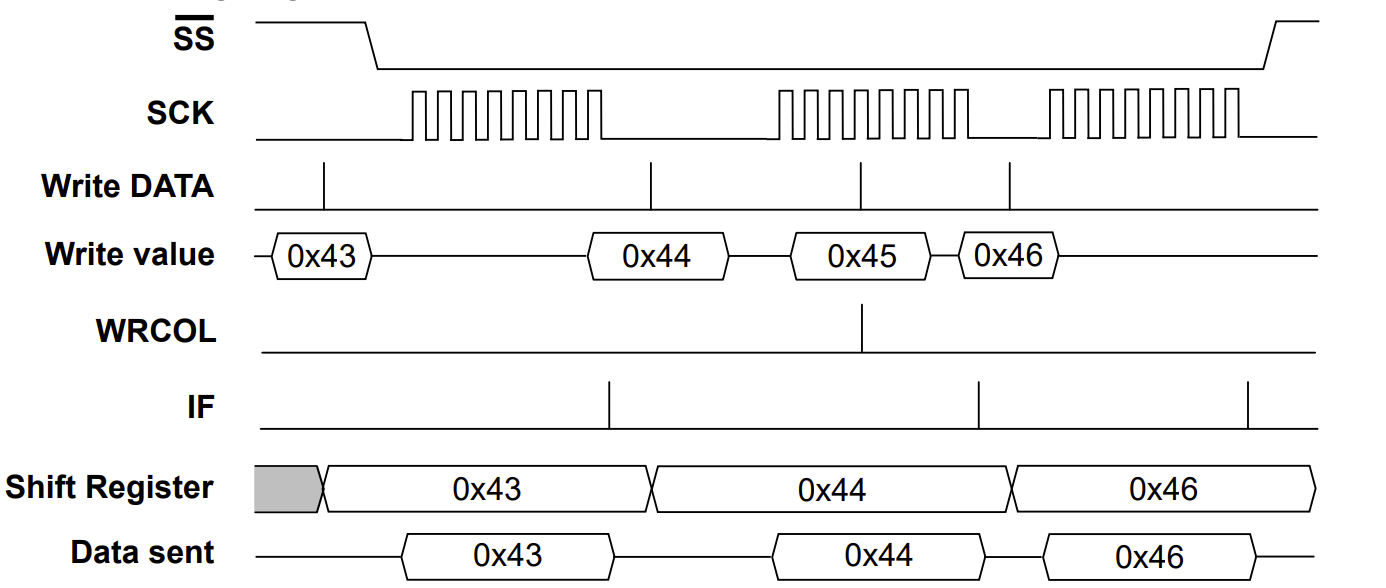
\includegraphics[width=0.85\textwidth]{images/spi_master_timing.png}
    \caption{Master Mode Timing Diagram}
    \label{fig:spi_master_timing}
\end{figure}

\subsubsection{Normal Mode}
In normal mode without buffering:

\begin{itemize}
    \item \textbf{Transmission starts immediately after writing to \texttt{DATA}.}
    \item \textbf{The core is single-buffered for transmission and double-buffered for reception.}
    \item \textbf{The Write Collision flag (\texttt{WRCOL}) is set if \texttt{DATA} is written before a transmission completes.}
\end{itemize}

\subsubsection{Buffer Mode}
Enabling buffer mode provides additional buffering:

\begin{itemize}
    \item \textbf{Double-buffered transmission and triple-buffered reception.}
    \item \textbf{Allows writing to \texttt{DATA} while a transmission is ongoing.}
    \item \textbf{Use the Data Register Empty Interrupt Flag (\texttt{DREIF}) to check if \texttt{DATA} can be written.}
\end{itemize}

% Buffer Mode Diagram
\begin{figure}[H]
    \centering
    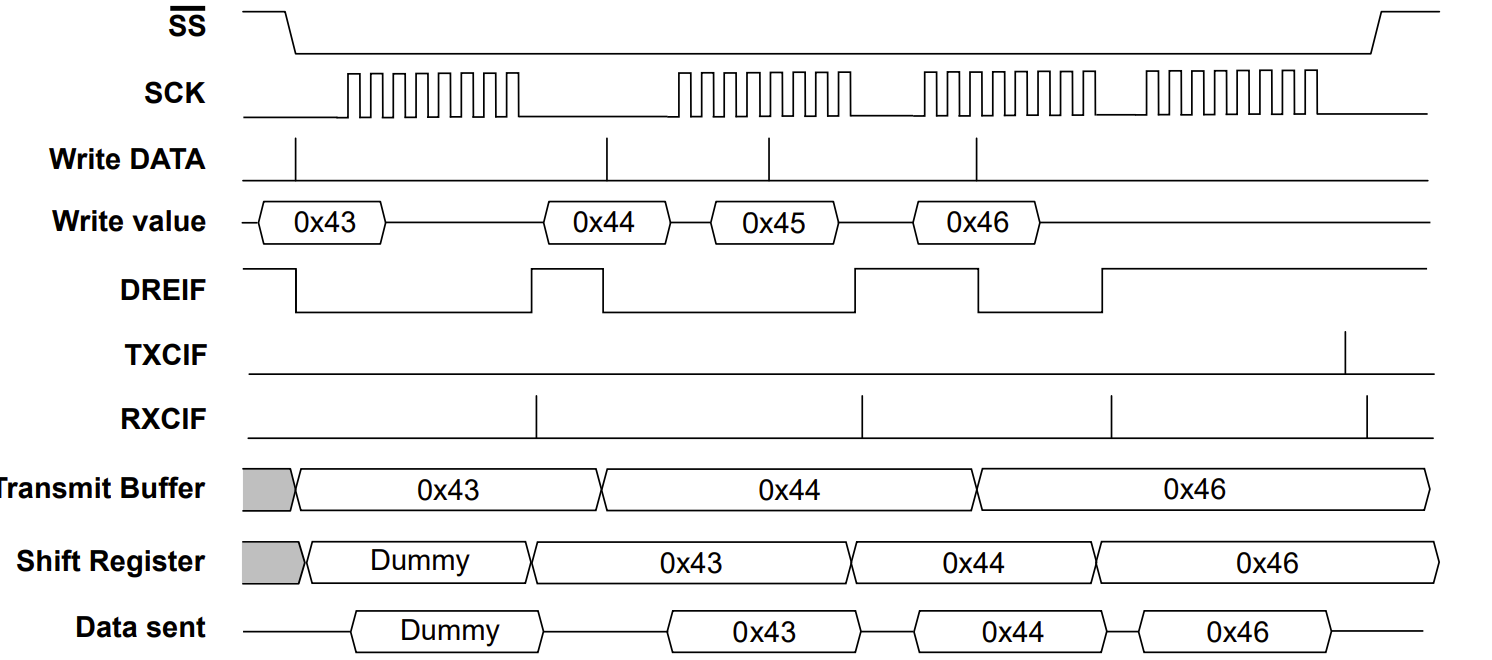
\includegraphics[width=0.85\textwidth]{images/spi_buffer_mode.png}
    \caption{SPI Buffer Mode Operation}
    \label{fig:spi_buffer_mode}
\end{figure}

\subsection{Slave Mode}
In slave mode, the SPI core operates passively, awaiting instructions from the master device. It does not generate the clock signal but instead responds to the master's SCK and SS signals.

\subsubsection{Normal Mode}
Operating in normal mode without buffering involves the following characteristics:

\begin{itemize}
    \item \textbf{Initiated by Master:} Transmission and reception are controlled by the master device, which dictates when data transfers occur.
    \item \textbf{Data Preparation:} Data must be written to the Data Register (\texttt{DATA}) before the master initiates a transfer. Failure to do so can result in incomplete or corrupted data transmission.
    \item \textbf{Write Collision Detection:} Similar to master mode, if \texttt{DATA} is written during an ongoing transfer, the Write Collision flag (\texttt{WRCOL}) is set, indicating a collision.
\end{itemize}

\subsubsection{Buffer Mode}
Buffer mode in slave operation offers enhanced data handling capabilities:

\begin{itemize}
    \item \textbf{Pre-Buffered Transmission:} Allows the slave to prepare multiple bytes of data in advance, ensuring seamless data transmission when the master initiates a transfer.
    \item \textbf{Graceful Overrun Handling:} Buffer mode can detect and manage data overruns, preventing data loss and maintaining system stability.
    \item \textbf{Configurable Buffer Behavior:} The Buffer Mode Wait for Receive (\texttt{BUFWR}) bit in \texttt{CTRLB} allows configuration of how the buffer behaves during data reception, enabling flexible data handling strategies.
\end{itemize}

% Slave Mode Timing Diagram
\begin{figure}[H]
    \centering
    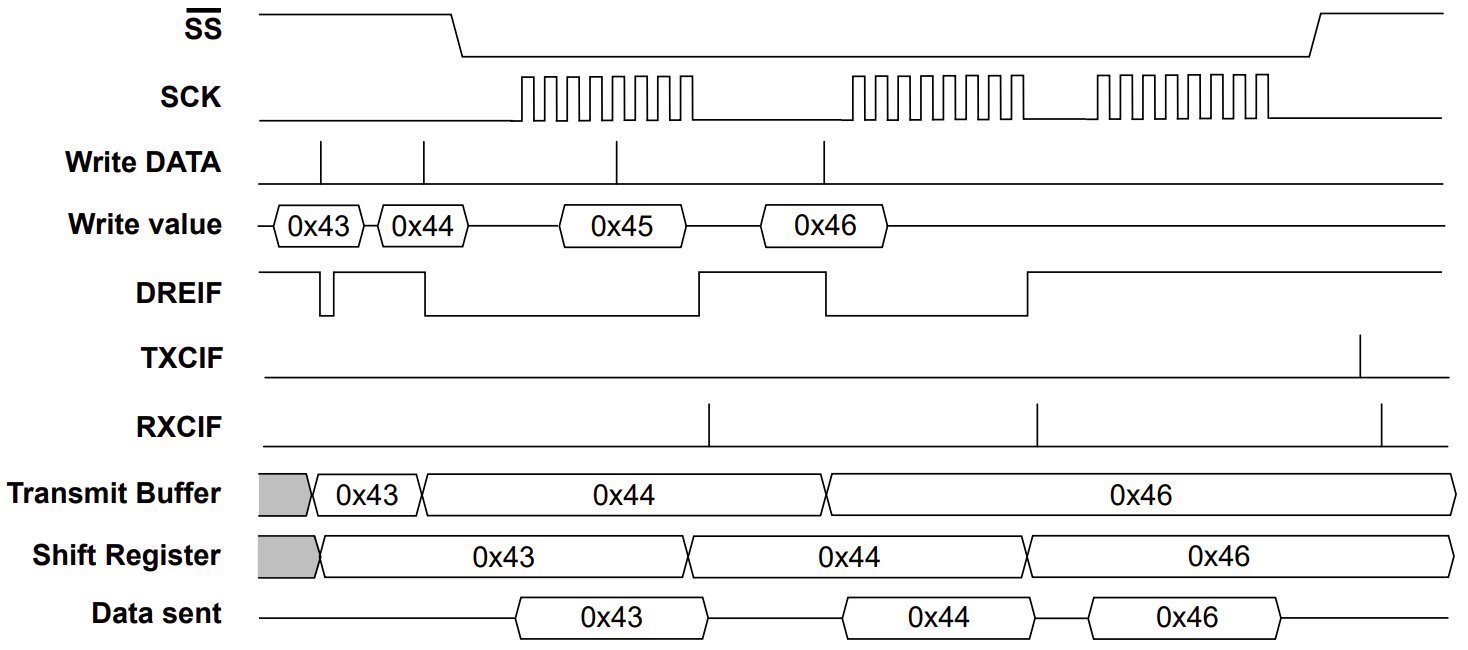
\includegraphics[width=0.85\textwidth]{images/spi_slave_timing.png}
    \caption{Slave Mode Timing Diagram}
    \label{fig:spi_slave_timing}
\end{figure}

\subsubsection{Normal Mode}
In normal mode:

\begin{itemize}
    \item \textbf{Transmission begins when SS is low and SCK pulses are received.}
    \item \textbf{Data must be written to \texttt{DATA} before the master initiates a transfer.}
    \item \textbf{The Write Collision flag (\texttt{WRCOL}) is set if \texttt{DATA} is written during an ongoing transfer.}
\end{itemize}

\subsubsection{Buffer Mode}
Buffer mode in slave operation allows for:

\begin{itemize}
    \item \textbf{Preparing data in advance for transmission.}
    \item \textbf{Handling data overruns more gracefully.}
    \item \textbf{Configurable behavior using the Buffer Mode Wait for Receive (\texttt{BUFWR}) bit.}
\end{itemize}

% % Slave Buffer Mode Diagram
% \begin{figure}[H]
%     \centering
%     \includegraphics[width=0.85\textwidth]{images/spi_slave_buffer_mode.png}
%     \caption{Slave Buffer Mode Operation}
%     \label{fig:spi_slave_buffer_mode}
% \end{figure}

\section{Data Transfer Modes}
The SPI protocol defines four distinct data transfer modes, each determined by the Clock Polarity (CPOL) and Clock Phase (CPHA). These modes dictate the timing relationship between the clock signal and data signals, ensuring synchronized and accurate data transmission.

\begin{table}[H]
    \centering
    \caption{SPI Data Transfer Modes}
    \begin{tabular}{@{}ccc@{}}
        \toprule
        \textbf{Mode} & \textbf{CPOL} & \textbf{CPHA} \\ \midrule
        0 & 0 & 0 \\
        1 & 0 & 1 \\
        2 & 1 & 0 \\
        3 & 1 & 1 \\ \bottomrule
    \end{tabular}
    \label{tab:spi_modes}
\end{table}

\begin{itemize}
    \item \textbf{Mode 0 (CPOL=0, CPHA=0):} 
    \begin{itemize}
        \item \textbf{Clock Polarity (CPOL):} The clock signal (SCK) is low when idle.
        \item \textbf{Clock Phase (CPHA):} Data is sampled on the leading (rising) edge of the clock.
        \item \textbf{Description:} Data is set up on the trailing edge and sampled on the leading edge, ensuring data stability before sampling.
    \end{itemize}
     
    \item \textbf{Mode 1 (CPOL=0, CPHA=1):}
    \begin{itemize}
        \item \textbf{Clock Polarity (CPOL):} The clock signal (SCK) is low when idle.
        \item \textbf{Clock Phase (CPHA):} Data is sampled on the trailing (falling) edge of the clock.
        \item \textbf{Description:} Data is set up on the leading edge and sampled on the trailing edge, providing flexibility in data timing.
    \end{itemize}
    
    \item \textbf{Mode 2 (CPOL=1, CPHA=0):}
    \begin{itemize}
        \item \textbf{Clock Polarity (CPOL):} The clock signal (SCK) is high when idle.
        \item \textbf{Clock Phase (CPHA):} Data is sampled on the leading (falling) edge of the clock.
        \item \textbf{Description:} Data is set up on the trailing edge and sampled on the leading edge, suitable for systems where a high idle clock state is preferred.
    \end{itemize}
    
    \item \textbf{Mode 3 (CPOL=1, CPHA=1):}
    \begin{itemize}
        \item \textbf{Clock Polarity (CPOL):} The clock signal (SCK) is high when idle.
        \item \textbf{Clock Phase (CPHA):} Data is sampled on the trailing (rising) edge of the clock.
        \item \textbf{Description:} Data is set up on the leading edge and sampled on the trailing edge, allowing for alternate data sampling strategies.
    \end{itemize}
\end{itemize}

% Data Transfer Modes Timing Diagrams
\begin{figure}[H]
    \centering
    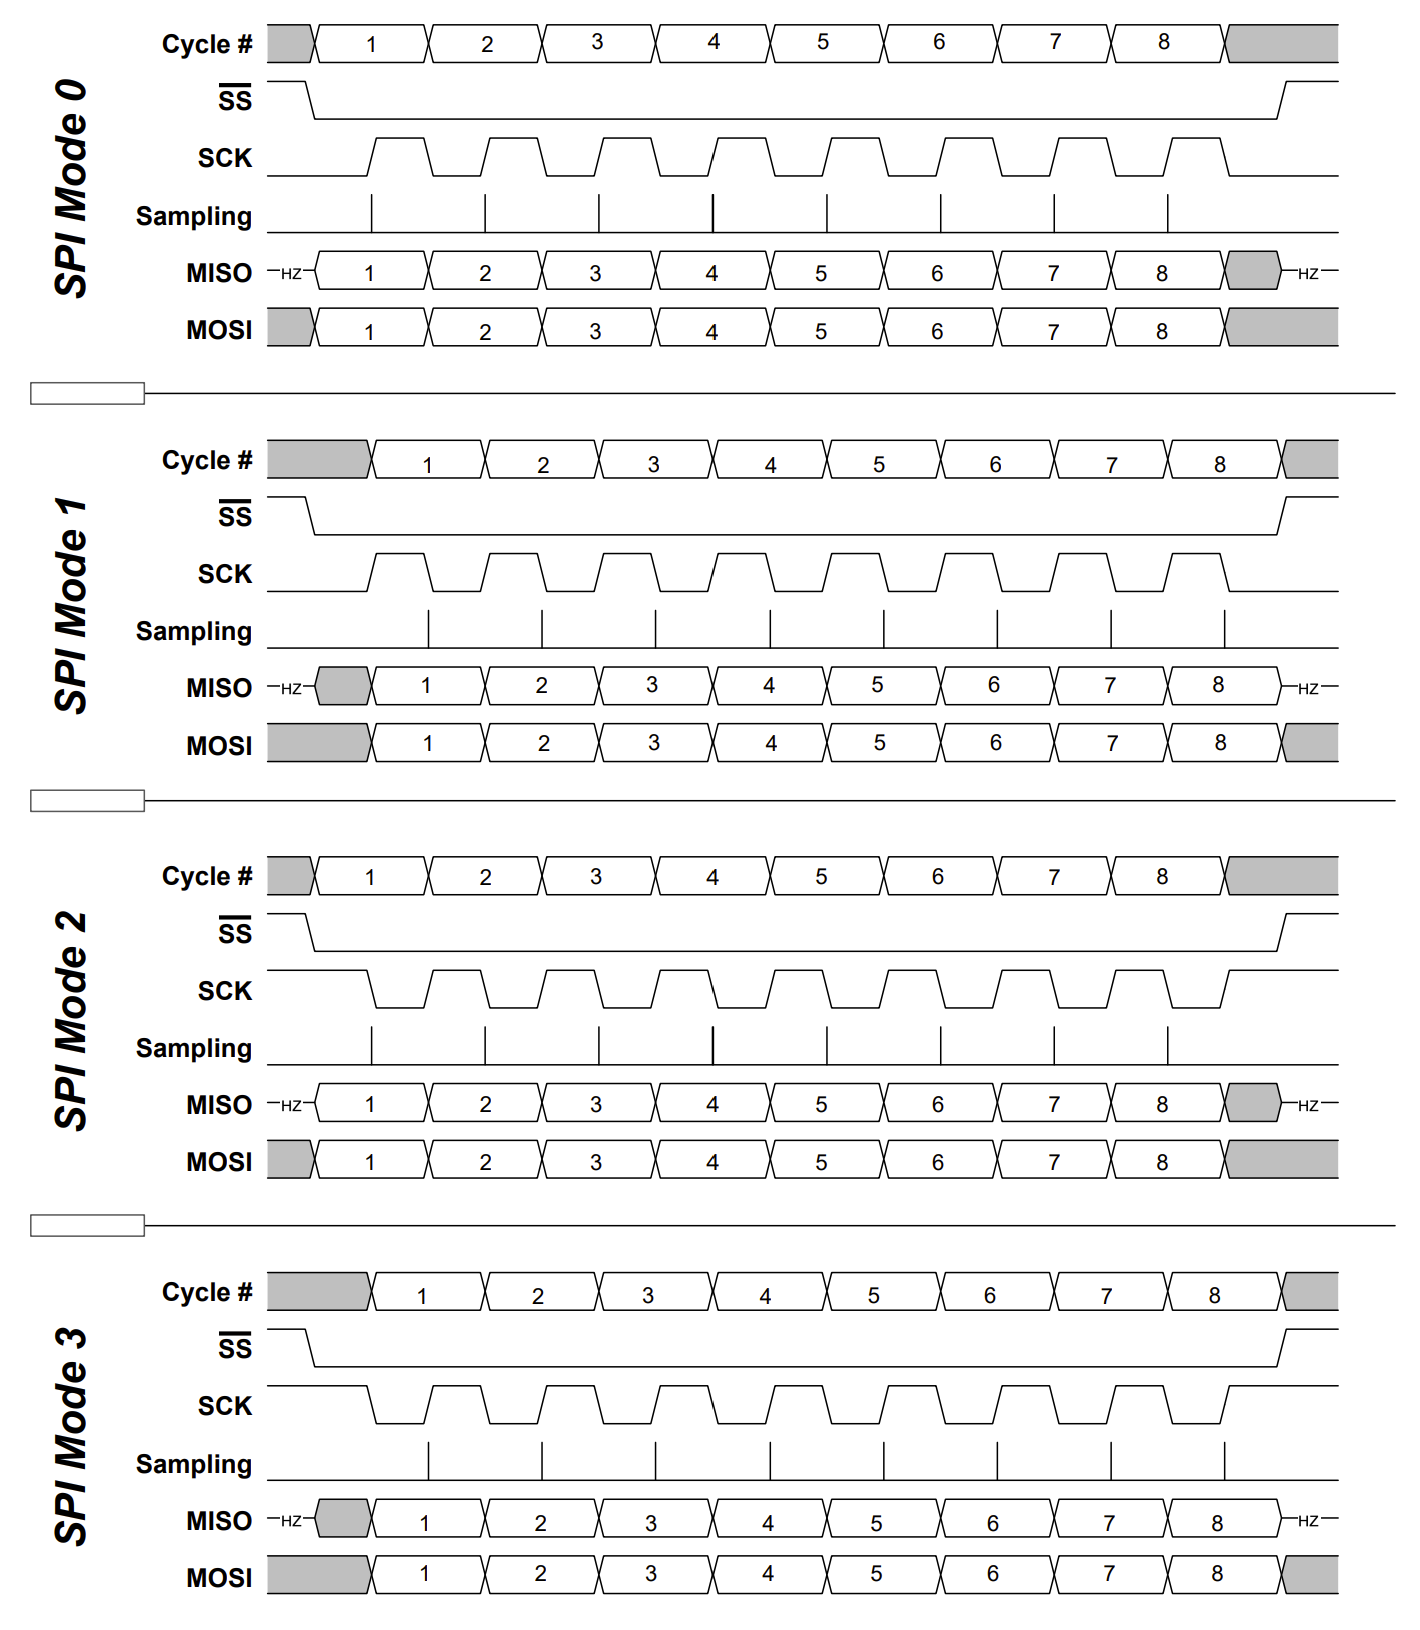
\includegraphics[width=0.9\textwidth]{images/spi_data_modes.png}
    \caption{SPI Data Transfer Modes Timing Diagrams}
    \label{fig:spi_data_modes}
\end{figure}

\subsection{Impact of CPOL and CPHA}
Understanding the interplay between CPOL and CPHA is essential for configuring the SPI core correctly:

\begin{itemize}
    \item \textbf{Clock Polarity (CPOL):} Determines the idle state of the clock signal. A CPOL of \texttt{0} means the clock is low when idle, while a CPOL of \texttt{1} means it is high.
    \item \textbf{Clock Phase (CPHA):} Determines on which clock edge data sampling occurs. A CPHA of \texttt{0} means data is sampled on the leading edge, and a CPHA of \texttt{1} means it is sampled on the trailing edge.
\end{itemize}

\subsection{Selecting the Appropriate Mode}
Choosing the correct SPI mode is crucial for ensuring compatibility between master and slave devices. Mismatched modes can lead to data corruption or communication failures. It's important to consult the datasheets of all connected devices to determine the appropriate CPOL and CPHA settings.

\section{Interrupts}
The SPI core leverages interrupt mechanisms to handle various events efficiently, allowing the system to respond promptly to data transmission and reception without constant polling.

\subsection{Interrupt Types}
The SPI core provides multiple interrupt flags and enables to manage different events:

\begin{itemize}
    \item \textbf{Interrupt Flag (\texttt{IF}):} Indicates that a data transfer has been completed.
    \item \textbf{Write Collision (\texttt{WRCOL}):} Signals that a write attempt to the Data Register (\texttt{DATA}) occurred while a transfer was still in progress.
    \item \textbf{Receive Complete (\texttt{RXCIF}):} Indicates that data reception is complete in buffer mode.
    \item \textbf{Transfer Complete (\texttt{TXCIF}):} Signals that data transmission is complete and the transmit buffer is empty in buffer mode.
    \item \textbf{Data Register Empty (\texttt{DREIF}):} Indicates that the \texttt{DATA} register is ready to accept new data in buffer mode.
    \item \textbf{Slave Select Trigger (\texttt{SSIF}):} Notifies that the SS line has been asserted in buffer mode.
    \item \textbf{Buffer Overflow (\texttt{BUFOVF}):} Alerts that a buffer overflow has occurred in reception.
\end{itemize}

\subsection{Interrupt Enabling}
To utilize interrupts, the corresponding enable bits in the Interrupt Control Register (\texttt{INTCTRL}) must be set. This configuration allows the SPI core to generate interrupt requests based on specific events, facilitating responsive and efficient data handling.

\subsection{Interrupt Handling}
Upon the occurrence of an interrupt event, the system's interrupt service routine (ISR) should handle the event appropriately. For example:
\begin{itemize}
    \item \textbf{Data Transfer Completion:} The ISR can process the received data or prepare the next data byte for transmission.
    \item \textbf{Write Collision Detection:} The ISR can log the collision event and take corrective measures to prevent data corruption.
    \item \textbf{Buffer Overflow Handling:} The ISR can clear the overflow flag and implement strategies to manage data loss.
\end{itemize}

\subsection{Normal Mode vs. Buffer Mode Interrupts}
The Interrupt Flags Register (\texttt{INTFLAGS}) behaves differently based on whether the SPI core is operating in normal mode or buffer mode:

\subsubsection{Normal Mode Interrupts}
In normal mode, only the general Interrupt Flag (\texttt{IF}) and Write Collision Flag (\texttt{WRCOL}) are relevant. These flags notify the system of transfer completions and write collisions, respectively.

\subsubsection{Buffer Mode Interrupts}
In buffer mode, additional interrupt flags become active, providing finer control over data handling. These include flags for receive completion, transfer completion, data register emptiness, slave select triggers, and buffer overflows.

\subsection{Interrupt Timing}
Efficient interrupt handling ensures that the SPI core can manage data transfers without bottlenecks or data loss. Properly timed interrupts allow the system to handle high-throughput data streams seamlessly.

\section{Register Description}

\subsection{Control Register A (\texttt{CTRLA})}
\label{sec:ctrla}

\begin{table}[H]
    \centering
    \caption{Control Register A (\texttt{CTRLA})}
    \begin{tabular}{@{}cccccccc@{}}
        \toprule
        \textbf{Bit} & 7 & 6 & 5 & 4 & 3 & 2-1 & 0 \\ \midrule
        \textbf{Name} & DORD & MASTER & CLK2X & PRESC2 & PRESC1 & PRESC[1:0] & ENABLE \\ \bottomrule
    \end{tabular}
    \label{tab:ctrl_a}
\end{table}

\begin{itemize}
    \item \textbf{Bit 7 - DORD (Data Order):} 
    \begin{itemize}
        \item \texttt{0}: MSB (Most Significant Bit) transmitted first.
        \item \texttt{1}: LSb (Least Significant Bit) transmitted first.
    \end{itemize}
    \textit{Description:} This bit configures the order in which data bits are transmitted and received. Selecting LSb first can be beneficial for certain peripherals or communication protocols that prioritize lower-order bits.
    
    \item \textbf{Bit 6 - MASTER:} 
    \begin{itemize}
        \item \texttt{0}: Slave mode.
        \item \texttt{1}: Master mode.
    \end{itemize}
    \textit{Description:} Determines whether the SPI core operates as a master or a slave. In master mode, the core generates the clock and controls SS lines. In slave mode, it responds to the master's commands.
    
    \item \textbf{Bit 5 - CLK2X (Clock Double):} 
    \begin{itemize}
        \item \texttt{0}: SPI clock rate not doubled.
        \item \texttt{1}: SPI clock rate doubled.
    \end{itemize}
    \textit{Description:} When set, this bit doubles the SPI clock frequency after prescaling in master mode, effectively increasing data transfer speed.
    
    \item \textbf{Bit 4 - PRESC2:} 
    \begin{itemize}
        \item \texttt{0}: Prescaler bit 2 not set.
        \item \texttt{1}: Prescaler bit 2 set.
    \end{itemize}
    \textit{Description:} Part of the prescaler configuration that determines the division factor for the SPI clock.
    
    \item \textbf{Bit 3 - PRESC1:} 
    \begin{itemize}
        \item \texttt{0}: Prescaler bit 1 not set.
        \item \texttt{1}: Prescaler bit 1 set.
    \end{itemize}
    \textit{Description:} Another part of the prescaler configuration, working in conjunction with PRESC2 and PRESC[1:0] to set the overall clock division factor.
    
    \item \textbf{Bits 2-1 - PRESC[1:0] (Prescaler):} 
    \begin{itemize}
        \item \texttt{00}: Divide by 4.
        \item \texttt{01}: Divide by 16.
        \item \texttt{10}: Divide by 64.
        \item \texttt{11}: Divide by 128.
    \end{itemize}
    \textit{Description:} These bits define the base division factor applied to the peripheral clock to generate the SPI clock rate. Higher division factors result in lower SPI clock speeds.
    
    \item \textbf{Bit 0 - ENABLE:} 
    \begin{itemize}
        \item \texttt{0}: SPI disabled.
        \item \texttt{1}: SPI enabled.
    \end{itemize}
    \textit{Description:} Activates or deactivates the SPI core. Disabling the SPI core can save power when communication is not required.
\end{itemize}

\subsection{Control Register B (\texttt{CTRLB})}
\label{sec:ctrlb}

\begin{table}[H]
    \centering
    \caption{Control Register B (\texttt{CTRLB})}
    \begin{tabular}{@{}cccccccc@{}}
        \toprule
        \textbf{Bit} & 7 & 6 & 5 & 4 & 3 & 2-1 & 0 \\ \midrule
        \textbf{Name} & BUFEN & BUFWR & SSD & PRESC3 & PRESC2 & MODE[1:0] & Reserved \\ \bottomrule
    \end{tabular}
    \label{tab:ctrl_b}
\end{table}


\begin{itemize}
    \item \textbf{Bit 7 - BUFEN (Buffer Enable):} 
    \begin{itemize}
        \item \texttt{0}: Buffer mode disabled.
        \item \texttt{1}: Buffer mode enabled.
    \end{itemize}
    \textit{Description:} When set, enables buffer mode, allowing the SPI core to handle multiple data bytes efficiently through additional buffering mechanisms.
    
    \item \textbf{Bit 6 - BUFWR (Buffer Wait for Receive):} 
    \begin{itemize}
        \item \texttt{0}: Sends a dummy byte before user data.
        \item \texttt{1}: Sends user data immediately.
    \end{itemize}
    \textit{Description:} Configures the behavior of the buffer in slave mode. Setting this bit to \texttt{1} allows user data to be sent immediately upon transmission initiation, while \texttt{0} introduces a dummy byte to ensure data synchronization.
    
    \item \textbf{Bit 5 - SSD (Slave Select Disable):} 
    \begin{itemize}
        \item \texttt{0}: SS pin used for multi-master support.
        \item \texttt{1}: SS pin ignored; used as general I/O.
    \end{itemize}
    \textit{Description:} Controls the behavior of the SS pin in master mode. Disabling SS pin ensures that the master remains in control even if the SS pin is externally manipulated, which is crucial in multi-master environments.
    
    \item \textbf{Bit 4 - PRESC3:} 
    \begin{itemize}
        \item \texttt{0}: Prescaler bit 3 not set.
        \item \texttt{1}: Prescaler bit 3 set.
    \end{itemize}
    \textit{Description:} Part of the extended prescaler configuration, allowing for finer control over the SPI clock rate.
    
    \item \textbf{Bits 3-2 - PRESC2:} 
    \begin{itemize}
        \item \texttt{00}: Prescaler bits 3 and 2 not set.
        \item \texttt{01}: Prescaler bit 3 set, bit 2 not set.
        \item \texttt{10}: Prescaler bit 3 not set, bit 2 set.
        \item \texttt{11}: Both prescaler bits 3 and 2 set.
    \end{itemize}
    \textit{Description:} These bits work in conjunction with \texttt{PRESC[1:0]} to define a comprehensive prescaler value, allowing for a wide range of SPI clock rates.
    
    \item \textbf{Bits 1-0 - MODE[1:0] (Mode Selection):} 
    \begin{itemize}
        \item \texttt{00}: Mode 0.
        \item \texttt{01}: Mode 1.
        \item \texttt{10}: Mode 2.
        \item \texttt{11}: Mode 3.
    \end{itemize}
    \textit{Description:} Selects the SPI data transfer mode based on CPOL and CPHA settings, defining the timing relationship between the clock and data signals.
\end{itemize}

\subsection{Interrupt Control Register (\texttt{INTCTRL})}
\label{sec:intctrl}

\begin{table}[H]
    \centering
    \caption{Interrupt Control Register (\texttt{INTCTRL})}
    \begin{tabular}{@{}ccccccc@{}}
        \toprule
        \textbf{Bit} & 7 & 6 & 5 & 4 & 3-2 & 1-0 \\ \midrule
        \textbf{Name} & RXCIE & TXCIE & DREIE & SSIE & -- & IE \\ \bottomrule
    \end{tabular}
    \label{tab:intctrl}
\end{table}

\begin{itemize}
    \item \textbf{Bit 7 - RXCIE (Receive Complete Interrupt Enable):} 
    \begin{itemize}
        \item \texttt{0}: Receive Complete interrupt disabled.
        \item \texttt{1}: Receive Complete interrupt enabled.
    \end{itemize}
    \textit{Description:} When enabled, the SPI core generates an interrupt whenever data reception is complete in buffer mode, allowing the system to process the received data promptly.
    
    \item \textbf{Bit 6 - TXCIE (Transfer Complete Interrupt Enable):} 
    \begin{itemize}
        \item \texttt{0}: Transfer Complete interrupt disabled.
        \item \texttt{1}: Transfer Complete interrupt enabled.
    \end{itemize}
    \textit{Description:} Enables the generation of an interrupt when a data transmission cycle is complete in buffer mode, signaling that the transmit buffer is empty and ready for new data.
    
    \item \textbf{Bit 5 - DREIE (Data Register Empty Interrupt Enable):} 
    \begin{itemize}
        \item \texttt{0}: Data Register Empty interrupt disabled.
        \item \texttt{1}: Data Register Empty interrupt enabled.
    \end{itemize}
    \textit{Description:} When set, the SPI core issues an interrupt indicating that the \texttt{DATA} register is ready to accept new data for transmission. Writing new data to \texttt{DATA} clears this flag, either by writing the data or disabling the interrupt.
    
    \item \textbf{Bit 4 - SSIE (Slave Select Interrupt Enable):} 
    \begin{itemize}
        \item \texttt{0}: Slave Select Trigger interrupt disabled.
        \item \texttt{1}: Slave Select Trigger interrupt enabled.
    \end{itemize}
    \textit{Description:} Enables the generation of an interrupt when the Slave Select (SS) line is externally asserted in master mode, allowing the system to respond to external selection events.
    
    \item \textbf{Bit 0 - IE (Interrupt Enable):} 
    \begin{itemize}
        \item \texttt{0}: General interrupts in normal mode disabled.
        \item \texttt{1}: General interrupts in normal mode enabled.
    \end{itemize}
    \textit{Description:} Controls the overall interrupt functionality in normal mode. When set, the SPI core can generate interrupts based on the \texttt{IF} flag in normal mode.
\end{itemize}

\subsection{Interrupt Flags Register (\texttt{INTFLAGS})}
\label{sec:intflags}

The Interrupt Flags Register (\texttt{INTFLAGS}) monitors various interrupt conditions and flags. Its behavior varies depending on whether the SPI core is operating in normal mode or buffer mode.

\subsubsection{Normal Mode}
In normal mode, the \texttt{INTFLAGS} register contains the following flags:

\begin{table}[H]
    \centering
    \caption{Interrupt Flags Register (\texttt{INTFLAGS}) - Normal Mode}
    \begin{tabular}{@{}cc@{}}
        \toprule
        \textbf{Bit} & \textbf{Name} \\ \midrule
        7 & IF \\
        6 & WRCOL \\ \bottomrule
    \end{tabular}
    \label{tab:intflags_normal}
\end{table}

\begin{itemize}
    \item \textbf{Bit 7 - IF (Interrupt Flag):} 
    \begin{itemize}
        \item \texttt{0}: No interrupt.
        \item \texttt{1}: Interrupt flag set, indicating a data transfer has completed.
    \end{itemize}
    \textit{Description:} This flag is set automatically when a data transfer cycle is finished. It can be cleared by executing the corresponding interrupt vector or by reading the \texttt{INTFLAGS} register followed by accessing the \texttt{DATA} register.
    
    \item \textbf{Bit 6 - WRCOL (Write Collision Flag):} 
    \begin{itemize}
        \item \texttt{0}: No write collision detected.
        \item \texttt{1}: Write collision occurred, indicating an attempt to write to \texttt{DATA} during an ongoing transfer.
    \end{itemize}
    \textit{Description:} This flag alerts the system to potential data corruption caused by simultaneous write attempts. It must be cleared by first reading the \texttt{INTFLAGS} register and then accessing the \texttt{DATA} register.
\end{itemize}

\subsubsection{Buffer Mode}
In buffer mode, the \texttt{INTFLAGS} register encompasses additional flags to manage enhanced data handling:

\begin{table}[H]
    \centering
    \caption{Interrupt Flags Register (\texttt{INTFLAGS}) - Buffer Mode}
    \begin{tabular}{@{}cccccc@{}}
        \toprule
        \textbf{Bit} & 7 & 6 & 5 & 4 & 0 \\ \midrule
        \textbf{Name} & RXCIF & TXCIF & DREIF & SSIF & BUFOVF \\ \bottomrule
    \end{tabular}
    \label{tab:intflags_buffer}
\end{table}

\begin{itemize}
    \item \textbf{Bit 7 - RXCIF (Receive Complete Interrupt Flag):} 
    \begin{itemize}
        \item \texttt{0}: No data received.
        \item \texttt{1}: Data reception is complete.
    \end{itemize}
    \textit{Description:} Indicates that a byte of data has been successfully received and is available in the Receive Data Buffer register. Clearing this flag requires reading the \texttt{DATA} register or writing a \texttt{1} to the flag's bit position.
    
    \item \textbf{Bit 6 - TXCIF (Transfer Complete Interrupt Flag):} 
    \begin{itemize}
        \item \texttt{0}: Transfer not complete.
        \item \texttt{1}: Transfer complete and transmit buffer is empty.
    \end{itemize}
    \textit{Description:} Signals that all data in the transmit shift register has been shifted out, and there is no new data pending in the transmit buffer. This flag is cleared by writing a \texttt{1} to its bit position.
    
    \item \textbf{Bit 5 - DREIF (Data Register Empty Interrupt Flag):} 
    \begin{itemize}
        \item \texttt{0}: \texttt{DATA} register not ready for new data.
        \item \texttt{1}: \texttt{DATA} register is ready to accept new data.
    \end{itemize}
    \textit{Description:} Indicates that the \texttt{DATA} register is empty and ready to receive new data for transmission. Writing new data to \texttt{DATA} clears this flag, either by writing the data or disabling the interrupt.
    
    \item \textbf{Bit 4 - SSIF (Slave Select Interrupt Flag):} 
    \begin{itemize}
        \item \texttt{0}: SS line not asserted.
        \item \texttt{1}: SS line asserted.
    \end{itemize}
    \textit{Description:} This flag is set when the Slave Select (SS) line is externally asserted while the SPI core is in master mode. It can be cleared by writing a \texttt{1} to its bit position.
    
    \item \textbf{Bit 0 - BUFOVF (Buffer Overflow Flag):} 
    \begin{itemize}
        \item \texttt{0}: No buffer overflow.
        \item \texttt{1}: Buffer overflow detected.
    \end{itemize}
    \textit{Description:} Indicates that a buffer overflow has occurred during data reception, meaning the receive buffer was full when a new byte arrived. This flag is cleared by reading the \texttt{DATA} register or writing a \texttt{1} to its bit position.
\end{itemize}

\subsection{Data Register (\texttt{DATA})}
\label{sec:data_register}
The Data Register (\texttt{DATA}) serves as the primary interface for sending and receiving data through the SPI core. It is an 8-bit register, meaning it can hold one byte of data at a time.

\begin{itemize}
    \item \textbf{Writing to \texttt{DATA}:}
    \begin{itemize}
        \item In \textbf{master mode}, writing a byte to \texttt{DATA} initiates the transmission process. The byte is shifted out via the MOSI line while simultaneously receiving data from the slave through the MISO line.
        \item In \textbf{slave mode}, writing to \texttt{DATA} prepares the data to be sent to the master during the next communication initiated by the master.
    \end{itemize}
    
    \item \textbf{Reading from \texttt{DATA}:}
    \begin{itemize}
        \item Reading from \texttt{DATA} retrieves the most recently received byte of data. In buffer mode, reading from \texttt{DATA} also clears the \texttt{RXCIF} flag, indicating that the data has been processed.
    \end{itemize}
    
    \item \textbf{Behavior in Different Modes:}
    \begin{itemize}
        \item \textbf{Normal Mode:}
        \begin{itemize}
            \item \texttt{DATA} writes go directly to the shift register for immediate transmission.
            \item \texttt{DATA} reads fetch data from the Receive Data register.
        \end{itemize}
        \item \textbf{Buffer Mode:}
        \begin{itemize}
            \item \texttt{DATA} writes are stored in the Transmit Data Buffer register, allowing for buffered transmission.
            \item \texttt{DATA} reads retrieve data from the Receive Data Buffer register, ensuring that multiple received bytes can be handled efficiently.
        \end{itemize}
    \end{itemize}
\end{itemize}

\section{Usage Considerations}

\subsection{Multi-Master Support}
The SPI core is designed to support multi-master configurations, where multiple master devices can coexist on the same SPI bus. In such setups, the Slave Select (SS) line plays a crucial role in arbitration:

\begin{itemize}
    \item \textbf{Arbitration Mechanism:} If two masters attempt to communicate simultaneously, the SS line helps in determining which master gains control of the bus.
    \item \textbf{SS Pin Behavior:} The Slave Select Disable (\texttt{SSD}) bit in \texttt{CTRLB} determines how the SPI core responds when another master asserts the SS line. If \texttt{SSD} is not set, asserting SS will switch the SPI core to slave mode, preventing data collisions.
\end{itemize}

% Multi-Master Diagram
% \begin{figure}[H]
%     \centering
%     \includegraphics[width=0.85\textwidth]{images/spi_multi_master.png}
%     \caption{SPI Multi-Master Configuration}
%     \label{fig:spi_multi_master}
% \end{figure}

\subsection{Slave Select Behavior}
The Slave Select (SS) pin is integral to SPI communication, acting as a handshake between the master and slave devices. Proper management of the SS line ensures reliable and orderly data exchanges:

\begin{itemize}
    \item \textbf{Activation:} When the SS pin is pulled low by the master, the corresponding slave device becomes active and ready to communicate.
    \item \textbf{Deactivation:} When the SS pin is high, the slave device remains inactive, ignoring any SCK pulses or data on the bus.
    \item \textbf{Tri-State Behavior:} Inactive slave devices typically tri-state their MISO lines to prevent bus contention.
\end{itemize}

\begin{table}[H]
    \centering
    \caption{SS Pin Behavior in Slave Mode}
    \begin{tabular}{@{}ccc@{}}
        \toprule
        \textbf{SS Pin Level} & \textbf{SPI State} & \textbf{MISO Pin} \\ \midrule
        High & Inactive & Tri-stated \\
        Low & Active & Driven by SPI \\ \bottomrule
    \end{tabular}
    \label{tab:ss_behavior}
\end{table}

\subsection{Data Order and Modes}
Consistency in data order and SPI mode between master and slave devices is paramount for successful communication:

\begin{itemize}
    \item \textbf{Data Order:} Both devices must agree on whether data is transmitted with the MSB first or LSb first. Mismatched data orders can lead to misinterpretation of data bytes.
    \item \textbf{SPI Mode:} The Clock Polarity (CPOL) and Clock Phase (CPHA) settings must match between master and slave. This ensures that data is sampled and shifted correctly relative to the clock edges.
\end{itemize}

\subsubsection{Selecting Compatible Settings}
To achieve reliable communication:
\begin{enumerate}
    \item Determine the SPI mode supported by the peripheral device (slave).
    \item Configure the SPI core's \texttt{CTRLA} and \texttt{CTRLB} registers to match the peripheral's CPOL and CPHA settings.
    \item Ensure that both devices are configured to use the same data order (MSB or LSb first).
\end{enumerate}

\section{Simulation}

\subsection{Tests}
The test bench generates a number (default is 50) configurations of the
DynamicFifo that are highly randomized. There are two flavors of tests:

\begin{itemize}
  \item {Directed tests that fill the FIFO with random data and then read back
        the results to verify that the read data matches the writted data.}
  \item {Lengthy random tests that are used to check odd combinations of
        configurations and to compile code coverage data.}
\end{itemize}

\subsection{Code coverage}
All inputs and outputs are checked to insure each toggle at least once. An error
will be thrown in case any port fails to toggle.

The only exception are the \emph{almostEmptyLevel} and \emph{almostFullLevel}
which are intended to be static during each simulation. These signals are
excluded from coverage checks.

\subsection{Running simulation}

Simulations can be run directly from the command prompt as follows:

\begin{verbatim}
  $ sbt "test"
\end{verbatim}

or from make as follows:

\texttt{\$ make test}

\subsection{Viewing the waveforms}

The simulation generates an FST file that can be viewed using a waveform viewer. The command to view the waveform is as follows:
\begin{verbatim}
  $ gtkwave ./out/test/Gpio.fst
\end{verbatim}

% chktex-file 44
\section{Synthesis}

\subsection{Area}

The DynamicFifo has been tested in a number of configurations and the following
results should be representative of what a user should see in their own
technology.

\renewcommand*{\arraystretch}{1.4}
\begin{longtable}[H]{
    | p{0.20\textwidth}
    | p{0.15\textwidth}
    | p{0.15\textwidth}
    | p{0.15\textwidth}
    | p{0.15\textwidth} |
  }
  \hline
  \textbf{Config Name}   &
  \textbf{externalRAM}   &
  \textbf{dataWidth}     &
  \textbf{fifoDepth}     &
  \textbf{Gates}           \\ \hline \hline

  small\_false\_8\_8     &
  false                  &
  8                      &
  8                      &
  769                      \\ \hline

  medium\_false\_32\_64  &
  false                  &
  32                     &
  64                     &
  19,283                   \\ \hline

  large\_false\_64\_256  &
  false                  &
  64                     &
  256                    &
  152,808                  \\ \hline

  small\_true\_64\_256   &
  true                   &
  64                     &
  256                    &
  355                      \\ \hline

  medium\_true\_128\_128 &
  true                   &
  128                    &
  128                    &
  477                      \\ \hline

  large\_true\_256\_2048 &
  true                   &
  256                    &
  2048                   &
  502                      \\ \hline
  \caption{Synthesis results}\label{table:area}
\end{longtable}

\subsection{SDC File}
An \texttt{.sdc} file is generated to provide synthesis and static timing
analysis tools guidance for synthesis.

The \texttt{DynamicFifo.sdc} file is emitted and found in the
\texttt{./syn} directory.

\subsection{Timing}

The following timing was extracted using the generated~.sdc files using the
Nangate 45nm free library.

\renewcommand*{\arraystretch}{1.4}
\begin{longtable}[H]{
    | p{0.20\textwidth}
    | p{0.08\textwidth}
    | p{0.12\textwidth}
    | p{0.13\textwidth}
    | p{0.15\textwidth}
    | p{0.15\textwidth} |
  }
  \hline
  \textbf{Config Name}   &
  \textbf{Period}        &
  \textbf{Duty Cycle}    &
  \textbf{Input Delay}   &
  \textbf{Output Delay}  &
  \textbf{Slack}           \\ \hline \hline

  small\_false\_8\_8     &
  5ns                    &
  50\%                   &
  20\%                   &
  20\%                   &
  2.93 (MET)               \\ \hline

  medium\_false\_32\_64  &
  5ns                    &
  50\%                   &
  20\%                   &
  20\%                   &
  2.69 (MET)               \\ \hline

  large\_false\_64\_256  &
  5ns                    &
  50\%                   &
  20\%                   &
  20\%                   &
  2.80 (MET)               \\ \hline

  small\_true\_64\_256   &
  5ns                    &
  50\%                   &
  20\%                   &
  20\%                   &
  2.80 (MET)               \\ \hline

  medium\_true\_128\_128 &
  5ns                    &
  50\%                   &
  20\%                   &
  20\%                   &
  2.70 (MET)               \\ \hline

  large\_true\_256\_2048 &
  5ns                    &
  50\%                   &
  20\%                   &
  20\%                   &
  2.77 (MET)               \\ \hline
  \caption{Static Timing Analysis results}\label{table:timing}
\end{longtable}

\subsection{Multicycle Paths}
None.

\end{document}
